\title{Embedded Systems Design Project\\Nvidia: HiL Simulation for Automated Driving}
\author{
        \textsc{\"{O}rn Arnar Karlsson}\\
        \textsc{Samuel Tanner Lindemer}\\
        \textsc{Tony Lundgren}\\
        \textsc{Bratislav Markovic}\\
        \textsc{Oskar N\"{a}slund}\\
        \textsc{Tofik Sonono}\\
        \textsc{Pratheek Unnikrishnan}
}
\date{\today}

\documentclass[12pt,twoside]{article}

\usepackage[paper=a4paper,dvips,top=1.5cm,left=1.5cm,right=1.5cm,
    foot=1cm,bottom=1.5cm]{geometry}

%\usepackage[T1]{fontenc}
%%\usepackage{pslatex}
\renewcommand{\rmdefault}{ptm}
\usepackage{mathptmx}
\usepackage{amsmath}
\usepackage[scaled=.90]{helvet}
\usepackage{courier}
\usepackage{colortbl}
\usepackage{multirow}
\usepackage{bookmark}

\usepackage{fancyhdr}
\pagestyle{fancy}

%%----------------------------------------------------------------------------
%%   pcap2tex stuff
%%----------------------------------------------------------------------------
 \usepackage[dvipsnames*,svgnames]{xcolor} %% For extended colors
 \usepackage{tikz}
 \usetikzlibrary{arrows,decorations.pathmorphing,backgrounds,fit,positioning,calc,shapes}

%% \usepackage{pgfmath}	% --math engine
%%----------------------------------------------------------------------------
%% \usepackage[latin1]{inputenc}
\usepackage[utf8]{inputenc} % inputenc allows the user to input accented characters directly from the keyboard
\usepackage[swedish,english]{babel}
%% \usepackage{rotating}		 %% For text rotating
\usepackage{array}			 %% For table wrapping
\usepackage{graphicx}	                 %% Support for images
\usepackage{float}			 %% Suppor for more flexible floating box positioning
\usepackage{color}                       %% Support for colour
\usepackage{mdwlist}
%% \usepackage{setspace}                 %% For fine-grained control over line spacing
%% \usepackage{listings}		 %% For source code listing
%% \usepackage{bytefield}                %% For packet drawings
\usepackage{tabularx}		         %% For simple table stretching
%%\usepackage{multirow}	                 %% Support for multirow colums in tables
\usepackage{dcolumn}	                 %% Support for decimal point alignment in tables
\usepackage{url}	                 %% Support for breaking URLs
\usepackage[perpage,para,symbol]{footmisc} %% use symbols to ``number'' footnotes and reset which symbol is used first on each page

\usepackage{algorithm}
\usepackage{algorithmic}

%% \usepackage{pygmentize}           %% required to use minted -- see python-pygments - Pygments is a Syntax Highlighting Package written in Python
%% \usepackage{minted}		     %% For source code highlighting

%% \usepackage{hyperref}
%\usepackage[all]{hypcap}	 %% Prevents an issue related to hyperref and caption linking
\usepackage{caption}        %% Outclasses ^
%% setup hyperref to use the darkblue color on links
%% \hypersetup{colorlinks,breaklinks,
%%             linkcolor=darkblue,urlcolor=darkblue,
%%             anchorcolor=darkblue,citecolor=darkblue}

%% Some definitions of used colors
\definecolor{darkblue}{rgb}{0.0,0.0,0.3} %% define a color called darkblue
\definecolor{darkred}{rgb}{0.4,0.0,0.0}
\definecolor{red}{rgb}{0.7,0.0,0.0}
\definecolor{lightgrey}{rgb}{0.8,0.8,0.8}
\definecolor{grey}{rgb}{0.6,0.6,0.6}
\definecolor{darkgrey}{rgb}{0.4,0.4,0.4}
%% Reduce hyphenation as much as possible
\hyphenpenalty=15000
\tolerance=1000

%% useful redefinitions to use with tables
\newcommand{\rr}{\raggedright} %% raggedright command redefinition
\newcommand{\rl}{\raggedleft} %% raggedleft command redefinition
\newcommand{\tn}{\tabularnewline} %% tabularnewline command redefinition

%% definition of new command for bytefield package
\newcommand{\colorbitbox}[3]{%
	\rlap{\bitbox{#2}{\color{#1}\rule{\width}{\height}}}%
	\bitbox{#2}{#3}}

%% command to ease switching to red color text
\newcommand{\red}{\color{red}}
%%redefinition of paragraph command to insert a breakline after it
\makeatletter
\renewcommand\paragraph{\@startsection{paragraph}{4}{\z@}%
  {-3.25ex\@plus -1ex \@minus -.2ex}%
  {1.5ex \@plus .2ex}%
  {\normalfont\normalsize\bfseries}}
\makeatother

%%redefinition of subparagraph command to insert a breakline after it
\makeatletter
\renewcommand\subparagraph{\@startsection{subparagraph}{5}{\z@}%
  {-3.25ex\@plus -1ex \@minus -.2ex}%
  {1.5ex \@plus .2ex}%
  {\normalfont\normalsize\bfseries}}
\makeatother

\setcounter{tocdepth}{3}	%% 3 depth levels in TOC
\setcounter{secnumdepth}{5}
%%%%%%%%%%%%%%%%%%%%%%%%%%%%%%%%%%%%%%%%%%%%%%%%%%%%%%%%%%%%%%%%%%%%
%% End of preamble
%%%%%%%%%%%%%%%%%%%%%%%%%%%%%%%%%%%%%%%%%%%%%%%%%%%%%%%%%%%%%%%%%%%%

\renewcommand{\headrulewidth}{0pt}
\lhead{MF2063, Fall 2018, Period 1-2}
\chead{Final Technical Report}
\rhead{\date{\today}}

\makeatletter
\let\ps@plain\ps@fancy
\makeatother

\setlength{\headheight}{15pt}

\usepackage{pdfpages}
\begin{document}

\begin{figure}
    \centering
    
\includegraphics{KTH.png}
    \caption*{}
\end{figure}

\maketitle
\selectlanguage{english}

\begin{abstract}
%The abstract should be understandable without reading the whole report (and the
%whole report should be understandable without reading the abstract).
%Aim for about half a page of text outlining:
%The problem / issue / subject being addressed
%How the problem is tackled
%Overview of the results, and indication as to what level they solve the problem.
%Implications of the results
\end{abstract}
\clearpage

\tableofcontents
\clearpage

\listoffigures
\listoftables
\section*{Nomenclature}
%Identify and define key concepts, abbreviations or phrases used throughout your report.
\begin{basedescript}{\desclabelstyle{\pushlabel}\desclabelwidth{10em}}
\item[a]                    First letter in the alphabet
\item[b]                    Second letter in the alphabet
\item[c]                    Third letter in the alphabet
\end{basedescript}
\clearpage

\section{Introduction}
\label{section:Introduction}

\subsection{Background}
\label{section:Background}
%Describe at least the same points raised in the Abstract, but give more
%information. Save the technical details for later as much as possible.
%Open with an opinion or other statement that "captures" the reader and
%motivates them to keep reading.
%Give the societal / industrial context for your project. What area / discipline(s) %are
%involved. Briefly state who the contractor / company is, and why they have
%asked for this particular problem to be tackled. Is there a wider impact or
%application (e.g. in other disciplines / areas) if the problem can be solved?
%Get to the point quite quickly and keep your text relevant, preferably not more
%than 1-2 pages for part 1.1. Remember this section is the “story” or “hook” to
%generate interest in your reading further – you can provide the more detailed
%information / technical specifications in the following section


\subsection{Project Description}
\label{section:ProjectDescription}
%Describe your problem formulation, goals, and motivation. What does the project
%strive to achieve? What are your goals? What will be the benefit / impact of the
%project?
%What should be delivered / executed by the project? What issues are most
%important?
%Is partial success still useful? Will contributions be made even if ultimately the
%final deliverable fails?
%What are your team’s strengths in this area? Do you have a unique or novel
%approach.
%Use this section to show the complexities of the problem and any context that needs to be considered when tackling it.

\subsection{Delimitation}
\label{section:Delimitation}
%Specify the delimitations for your team (i.e. any technicalities / key aspects /
%influences that make up the problem but which your project will not focus on).

\subsection{Readers Guide / Report Disposition}
\label{section:ReadersGuideReportDisposition}
%Here you should give the reader a brief explanation of what each part of the
%report says and does for the report, so that the reader gets a sense of the
%content of each chapter and what connects them. After reading this the structure
%of the report should be known and make sense to the reader. Also state what you
%have in your appendix. This part 1.4 of the report should be between 1⁄2-1 page
%long.
\subsubsection{Methodology}
\label{section:ReadersGuide_Methodology}
\subsubsection{Implementation}
\label{section:ReadersGuide_Implementation}
\subsubsection{Verification and Validation}
\label{section:ReadersGuide_VerificationAndValidation}
\subsubsection{Results}
\label{section:ReadersGuide_Results}
\subsubsection{Discussions and Conclusion}
\label{section:ReadersGuide_DiscussionsAndConclusion}
\subsubsection{Future Work}
\label{section:ReadersGuide_FutureWork}
\subsubsection{Appendices}
\label{section:ReadersGuide_Appendices}

\section{Literary Review and State of the Art}
\label{section:LiteraryReviewAndStateOfTheArt}
% This is the only part of the report that should provide a description of theory. It should include any theoretical aspects you judge to be important for the reader to understand this (and following) chapter(s). Reflect upon what is known already about the problem, and which areas are novel. Are there common problems, and how have they been addressed / solved to date?
% Here you can also briefly describe similar systems or projects, and explain how they relate (or not) to the current problem.
% This chapter will be as long as it needs to be, and it is up to you to structure it so that it makes sense for your topic/problem/project. When the reader have read this part he or she should be able to more or less anticipate (or at least not be surprised by) the start of the next chapter, your methodology.
% Remember, in regard to the learning goals this course is not about theory. We know that you know how to properly engineer an embedded system. Here you should offer evidence that you can also apply that knowledge. Of the learning goals in the course these are the ones that we believe will definitely be covered by this chapter:
% Goal 1. Apply knowledge and skills from earlier courses, as well as learn to acquire new ones on demand: You can for instance indicate which sources are new to you, and which are not; structure their relationships to show what you have learnt during the course; cross-reference to other parts of the report to show how you applied the knowledge you discuss to your problem; etc.

\section{Methodology}
\label{section:Methodology}
%Think: Engineering approaches, Tool-chains, Project management, etc.
% Specify and describe the methods, tools and techniques you have used to solve the problem(s) in your project.
% Motivate your choice of methods.  Are there any reasonable alternatives? While you are free to use any best practice approach to engineering and project management you see fit, you are not being assessed on your grasp of theory about these approaches – you will be graded according to your ability to for instance match a relevant approach to the problem at hand. After reading this chapter the reader should have a good sense why you used the chosen tools/methods/techniques - you have shown the reader your “toolbox” and what you made with it.
% Some tips on Figures:
% Make sure that you use the same terminology in your figures as you do in the text.
% Connect the figures clearly to your text. Think about where it is on the page.
% The figure caption should contain enough information to explain the context.
% Remember, in regard to the learning goals this course is not about theory. We know that you know how to properly engineer an embedded system. Here you should offer evidence that you can also apply that knowledge. Of the learning goals in the course these are the ones that we believe will definitely be covered by this chapter:
% Goal 3. Use professional tools and processes necessary for the development of embedded systems: You can for instance describe the pros and cons of using different off-the-shelf platforms to solve your problem; indicate which tools (e.g. code checkers) you have used to solve/avoid issues that would typically emerge with the problem at hand; how different tools link up to provide important support during your development towards solving your problem; etc.
% Goal 4. Learn to get organised, manage, lead and become part of a cross technical and complex development project: You can for instance provide evidence of defining a proper scope for your project (such as a Product Breakdown Structure (PBS) and/or Work Breakdown Structure), using a risk management process (such as excerpts from a risk register), discussing which configuration management was important to your problem (such as the version control applied to which parts of the PBS), using quality control and quality assessment procedures (such as when and how reviews were made and the quality criteria of your products), properly raising issues with your project sponsor, etc.
% Goal 5. The student should after the course have good technical understanding, knowledge and skill in methods and tools for co-design and optimization of embedded systems: You can for instance discuss why a particular co-design/optimization method is appropriate for the problem at hand; identify which and how the different steps in your methodology are affected by the choice of method; cross-reference to other parts of the report to prove the impact of the method usage; etc. If you have not used any co-design or optimization method you are expected to at least argue for why this was not needed. Furthermore, in this case you are expected to discuss what other contemporary best practice methods suits your problem, and similarly provide evidence in regard to their proper use.
% Goal 6. Working through all aspects of an engineering development process: You can for instance show how to properly go from goals/limitations to requirements for your problem; how to make sure your requirements cover all relevant aspects (i.e. not only operations but also e.g. system disposal), how to identify and prioritise requirements; how to justify and clarify requirements with the project sponsor; etc.
% Goal 8. Being part of a larger engineering project, the student will learn how to apply a model-based development approach to embedded system development: As per Goal 5, but for model-based development.
% Goal 10. Apply a requirements management method with consideration taken to the life-cycle concerns of embedded systems based products: As per Goal 6, but specifically keep in mind that you need to provide evidence that you understand the context in which you develop your embedded system. As an example, applying machine learning to a robot could at a first glance seem like a standard problem with a model solution for a software engineer. However, the environmental conditions (fire, cold, dust, etc.) or special requirements (low weight, low power, etc.) of a use case can easily imply special sensing or actuating hardware, which in turn affect the requirements even on software. Furthermore, even if this is not the case, a proper engineering approach involves at least arguing for the non-existence of such requirements.


\subsection{Vector Maps}
At the outset of the project, the stakeholder's stated requirement was an automated process for generating an Autoware-compatible vector map for any PreScan simulation. The stakeholder was previously using a labor-intensive approximation method which only generated a very small subset of the vector map.

\subsubsection{Requirements Elicitation and Specification}
The project group attended a day-long seminar with a TASS International representative to establish alternatives. Four possible approaches were established.
\begin{enumerate}
  \item \textbf{Approach currently used by stakeholder:} Manually set a simulated vehicle to traverse every roadway. Save the location data to a file. (It was stipulated that this process could be automated.)
  \item \textbf{Approach recommended by TASS International:} Write scripts to automate PreScan's lane detection sensor. Scan the entire road map and save the sensor data to a file.
  \item Take screen captures of the road map and use image recognition methods to approximate the roads.
  \item \textbf{Approach chosen by project group:} Reverse-engineer PreScan’s internal road generation methods, as well as its undocumented simulation configuration file.
\end{enumerate}
Options 1 through 3 were identified as the most expedient approaches to the problem, as the developers could capture the road curvatures and dimensions without necessarily understanding anything about PreScan's internal logic. However, these naive approaches came with the risk that future updates to PreScan's MATLAB user interface or sensor definitions would render them inoperable.

It was decided that the feasibility of Option 4 should be investigated before proceeding. PreScan's XML-formatted configuration file is not documented for developers, and TASS International was unable to provide us any other API to directly access the road configurations. The configuration file contains a list of attributes defining road orientations and dimensions, but the methods and equations for generating the roads are not documented anywhere. These would have to be derived through experimentation. To complicate things further, it was discovered that the attributes listed in the configuration file only define the curvature of the road center lines, but the vector map requires separate curves for the center, lanes and road edges.

Thus, the configuration file approach presented both the highest development risk and the highest reward. The risk in pursuing this approach was the possibility that accurately deriving the complete road definition would not be possible within the time frame. The reward in pursuing this approach was producing a software package package requiring only a single input file which would be resilient to future PreScan updates. (It was judged highly unlikely that PreScan would completely overhaul their configuration file structure in a future software update.) Weighing these risks and benefits, the group concluded that this option was the best approach. After assessing the scale of this sub-project, two group members, Örn and Samuel, decided to make vector maps their entire focus for the reimainder of the project.

\begin{figure}[ht]
    \centering
    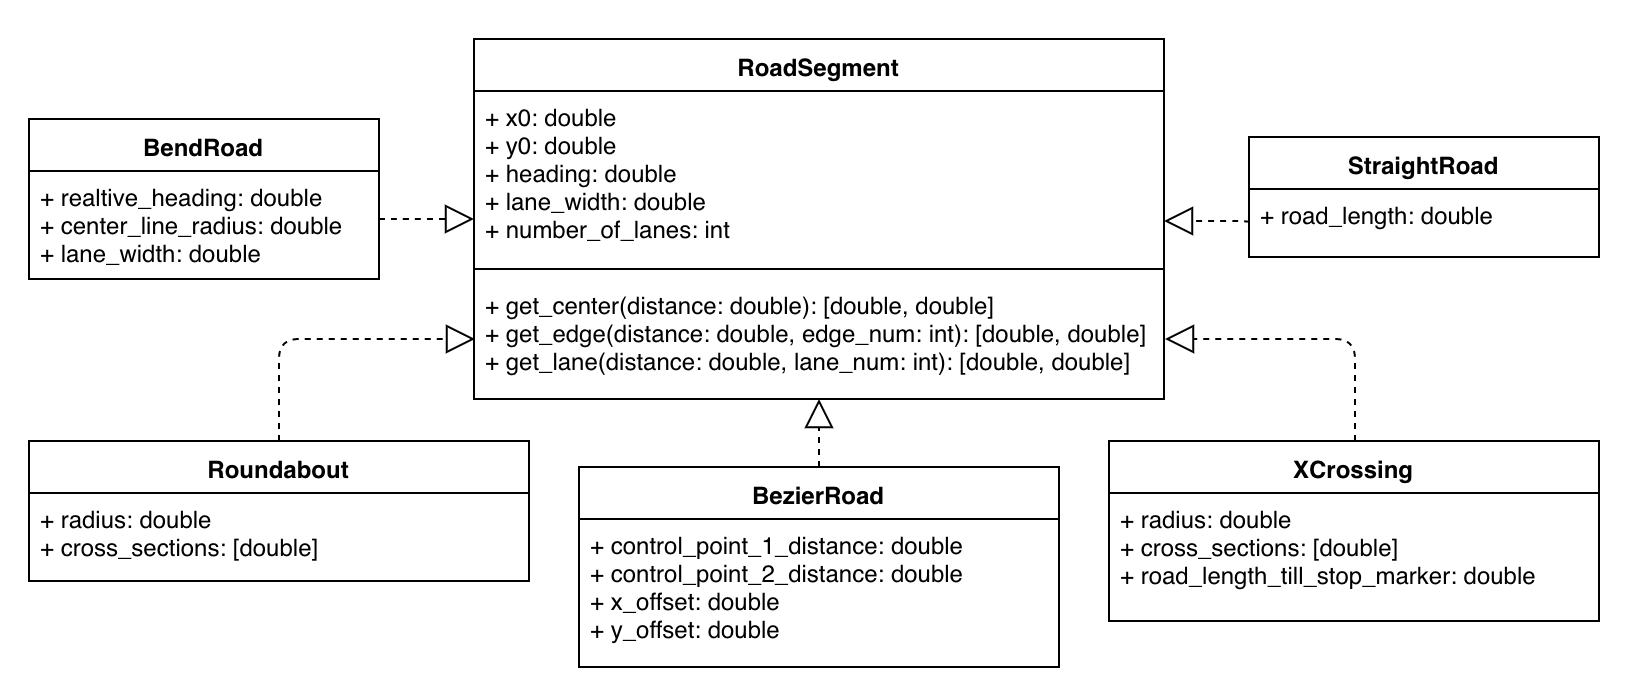
\includegraphics[width=18cm,keepaspectratio]{pex-uml.png}
    \caption{UML class diagram of road data in PreScan's configuration file. The bulk of the information defining the roads are in the algorithms used to generate them from these values. These algorithms are not accessible through the PreScan API.}
    \label{fig:pex-uml}
\end{figure}

\begin{figure}[ht]
    \centering
    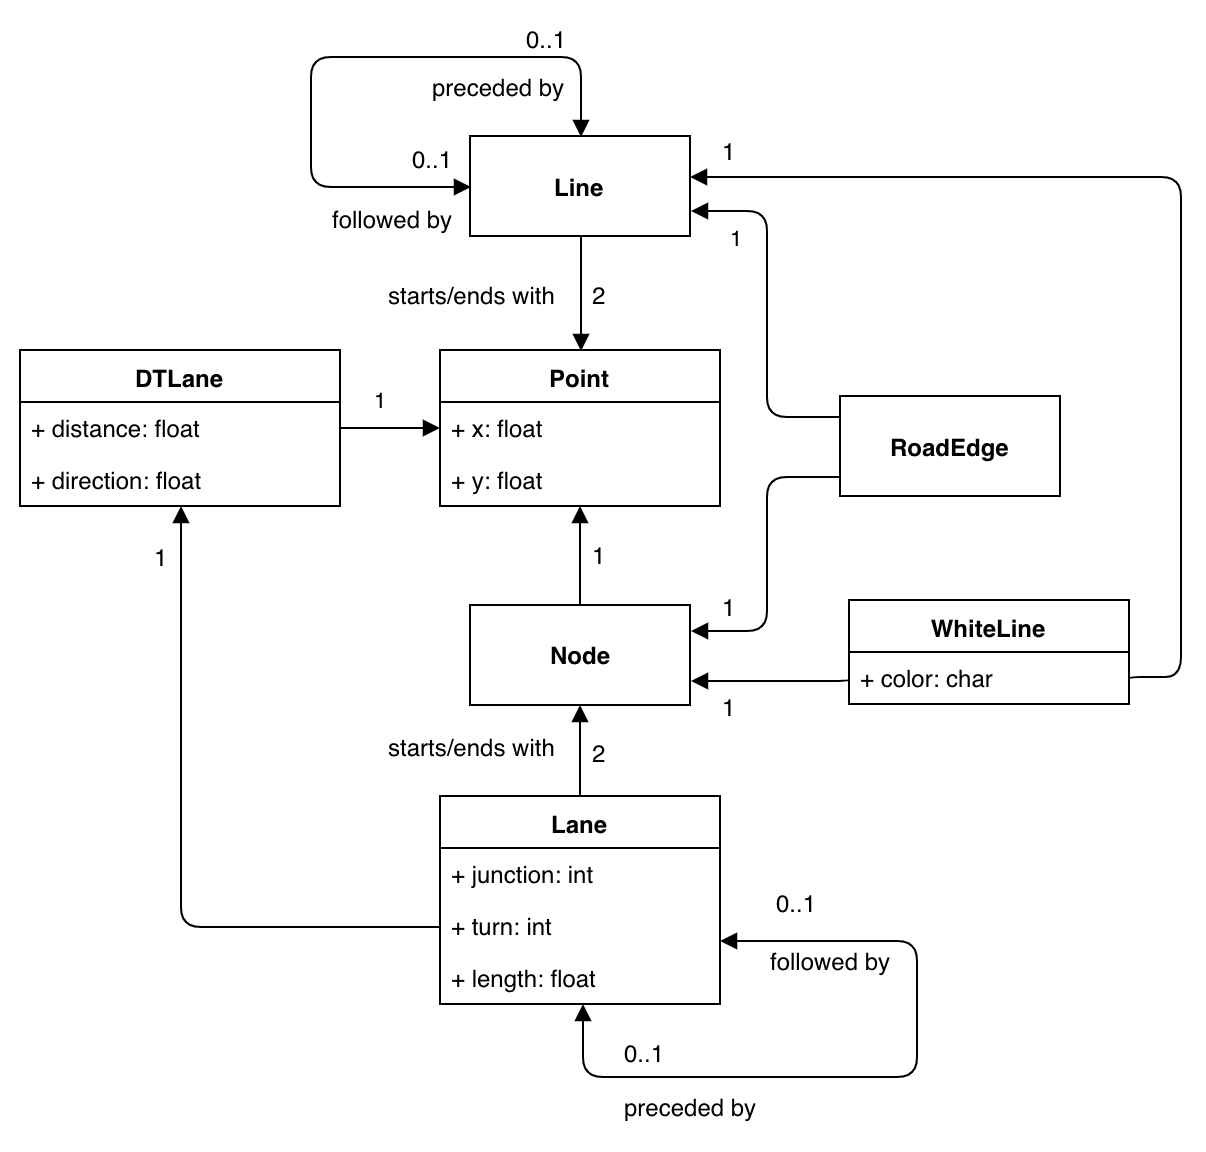
\includegraphics[width=12cm,keepaspectratio]{vmap-uml.png}
    \caption{UML class diagram of road data in the vector map format. Drivable lanes and other road features are defined as a sequence of linked coordinates. Each object in the above UML class diagram is represented as a single line in its corresponding CSV file.}
    \label{fig:vmap-uml}
\end{figure}

With the requirements adequately understood, two UML diagrams were drawn: one modeling the PreScan data represenation (see Figure \ref{fig:pex-uml}) and another modeling the vector map represenation (see Figure \ref{fig:vmap-uml}). The vector map data representation relies on coordinate data and the sequential relationships between them. The system of linking and sequncing every data point requires virtually complete knoweldge of the entire road system before the vector map can be generated. Unfortunately, there is no official documentation available for the vector map system.

\subsubsection{Agile and Extreme Programming (XP)}

It was clear in the early that the translation process would be fairly complex, and selecting an appropriate software development methodology would be crucial for a good result. It was apparent that our understanding of the system would evolve over time, and designing a complete software model without testing any code first would be difficult. This warranted an Agile software development approach, rather than a more rigid paradigm like the Waterfall or V-model framework. We chose Extreme Programming (XP) for its emphasis on pair programming, interaction and test-driven development. Here we present why we concluded this was the correct approach and how the principles and activities of XP concretely improved our design process.

\textbf{Pair programming.}
The early challenges we faced were largely based on mathematical problem solving. Solving these types of problems are often made easier when code can be used to assist dialog between problem solvers. Pair programming initial development steps followed a fairly simple system: one programmer would code a proposed algorithm on generating the roads until all the test input files could be parsed without errors. The results would be then be plotted for a visual comparison with the original roads in PreScan. The disparities would be discussed, and the keyboard would change hands.

With this process, many ineffective algorithms were ruled out in a matter of hours without duplicating work. The dialog between the two programmers kept the work flowing for hours at a time where a ``mental block'' would have been reached had the pair been working independently. Once all of the road models were being generated correctly, the two programmers each had a perfect understanding of how it all worked. The two were then able to quickly come to an agreement on where code could be reused and which interfaces were appropriate for the new classes.

\textbf{Stand-up meetings.}
These meetings incorporated members of the project group outside of the two programmers working directly on the vector mapping code. As the programmers justified design decisions on a whiteboard, other group members could offer a fresh perspective on a problem and point out incorrect assumptions or poor design choices. In one such meeting, Samuel explained that the latest version of the vector map generation code could take several minutes to run because every node had to be compared to ensure there were no duplicates. After the design choice that led to this was discussed, Tony demonstrated how clever use of hash tables would make this operation nearly instantaneous.

In another meeting, Örn and Samuel explained how three road models had already been derived without the use of high-level calculus, so no delays related to math should be expected. Oskar then pointed out that the Bezier road model that had been proposed was really only a rough approximation that would work for trivial cases. No test case had been written for non-trivial configurations of Bezier roads up to that point. Upon further research it was discovered that no analytical solution existed to this specific problem, and a numerical algorithm would have to be developed (see Section \ref{sec:vmap-coords}).

\textbf{Test-driven development.}
In XP, large problems are broken into smaller targets defined by a set of tests that the next code snippet must pass. This proved to be a huge aid for a pipelined data translation system such as this one. Any unexpected behavior could be narrowed down with a high degree of confidence to recently added code, not a cascade of effects from older code. One notable drawback to test-driven development in this project was that intial versions of code were typically done sub-optimally, probably because only black box unit tests were used.

The choice of XP as a development methodology influenced our decision to use Python instead of MATLAB. Python's third-party packages offer all the same functionality as MATLAB, plus a wider selection of testing and documentation packages. The \textit{pytest} package was chosen over the \textit{unittest} package found in the standard library. \textit{pytest} requires significantly less set-up and tear-down code to achieve the same outcome as \textit{unittest}. The online Python community largely seemed to agree that \textit{unittest} was designed for programmers familiar with JUnit and preferred to keep the same formalities (i.e., it uses camel case naming conventions which is not standard in Python).

\textbf{Summary.}
The activities in XP allowed the programmers in this project to quickly converge on well-justified design patterns for the software architecture. In the weekly stand-up meetings, the code segments written with the goal of passing unit tests were reviewed and adapted to conventional design patterns with agreed-upon interfaces. The iterator design pattern was used extensively in both the road generation and vector mapping subsystems in order to keep their complicated internal operation opaque to the rest of the system. The facade design pattern was used to isolate the vector mapping subsystem altogether, with only two simple interfaces to generate and link the entire map. Git version control was used throughout development, and the more modularized the code became, the easier it became for the programmers to collaborate without interfering in each others work.

\subsubsection{Documentation}
Concise documentation was absolutely necessary for the vector mapping code, as the stakeholder intended to expand its functionality over time and ultimately make it available to the public. Three options for Python were considered: \textit{Doxygen}, \textit{pdoc} and \textit{Sphinx}. All of these support automatic HTML and LaTeX documentation generation from comment strings in Python code, with \textit{pdoc} offering by far the simplest interface. \textit{Doxygen} is not Python-exclusive, and it has the most complicated interface, although it is an industry standard for languages like C++ and has been around a long time. Ultimately, \textit{Sphinx} was the best choice because Python itself uses it for documentation, so the resulting HTML docs will look familiar and accessible to any Python programmer (see Figure \ref{fig:doc-sample}). Only public functions are documented in the HTML docs. Other variables, classes and methods are documented with ordinary in-code comments. This way, the information relevant for users of the sofware subsystems is kept separate from those who want to edit them and add functionality.

\begin{figure}[ht]
    \centering
    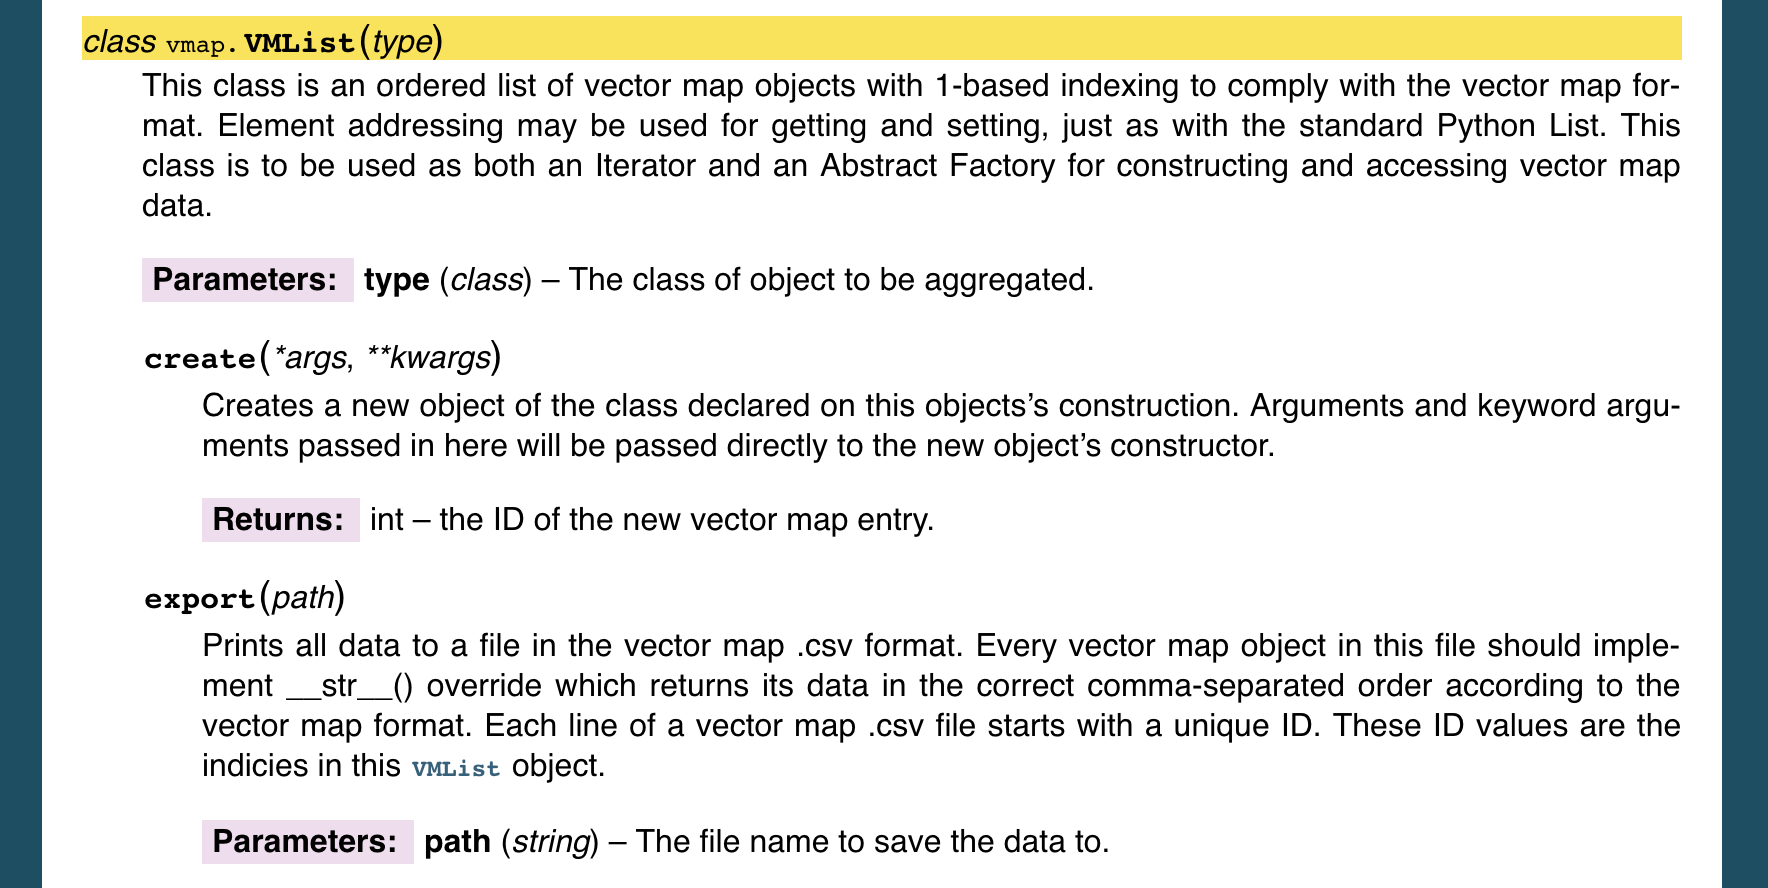
\includegraphics[width=16cm,keepaspectratio]{doc.png}
    \caption{Sample of the HTML documentation generated automatically from comment strings in the Python code using \textit{Sphinx}. This class uses the abstract factory design pattern: objects are created using the same generic interface regardless of their exact type. This class also implements the iterator design pattern, but that code is implemented with private override functions, so it does not appear in the HTML docs.}
    \label{fig:doc-sample}
\end{figure}

\section{Implementation}
\label{section:Implementation}
% Think: System overview, Models, Software, Hardware, Control, etc.
% Specify and describe the design and implementation of a system to address all or part of the goals of your project.
% Motivate your design and implementation. What were the reasonable design alternatives, and why did you choose this particular solution? After reading this chapter the reader should have a good sense of how you designed your system.
% Do not include results such as graphs, etc. (your results belong in the Results Section).
% Do not be too technically detailed. The idea is to provide an overview of the findings / system. You do not need to describe object methods, etc. in detail (unless they are new and decisive). Detailed information not critical to understanding the project and/or system should be included in an Appendix and referred to, rather than included in the body of your report. Doing this will enable a better flow for this chapter with a lower risk of the reader losing the thread.
% Remember, in regard to the learning goals this course is not about theory. We know that you know how to properly engineer an embedded system. Here you should offer evidence that you can also apply that knowledge. Of the learning goals in the course these are the ones that we believe will definitely be covered by this chapter:
% Goal 2.  Identify, compare and critically assess aspects of an engineering problem, towards making design decisions: You can for instance show you went from requirements to design alternatives for your problem; how you prioritised and chose between design alternatives; how you weighted different aspects of the design alternatives during your choices; how you justified your priorities and weighting in regard to design alternatives; etc.
% Goal 6. Working through all aspects of an engineering development process: As per Goal 2, but specifically keep in mind not only how your choices during design relate to requiremens but also to the verification and validation of your system.

\subsection{Vector Maps}
\subsubsection{Coordinate Generation}
\label{sec:vmap-coords}
PreScan uses three basic road types: \textit{StraightRoad} (implemented with a linear equation), \textit{BendRoad} (implemented with a semi circle) and \textit{BezierRoad} (implemented with a cubic Bezier curve). This much could be ascertained from the names of the road segments and their attributes in the configuration file. For the vector map, coordinates no more than 1 meter apart would need to be computed for the center of the roads, the center of the driving lanes, and the edges of the roads. The configuration file \textit{only} defines the center line curves, so algorithms for finding parallel curves for each equation based on the lane width was the next step.

\begin{figure}
\centering
\begin{tabular}{cc}
  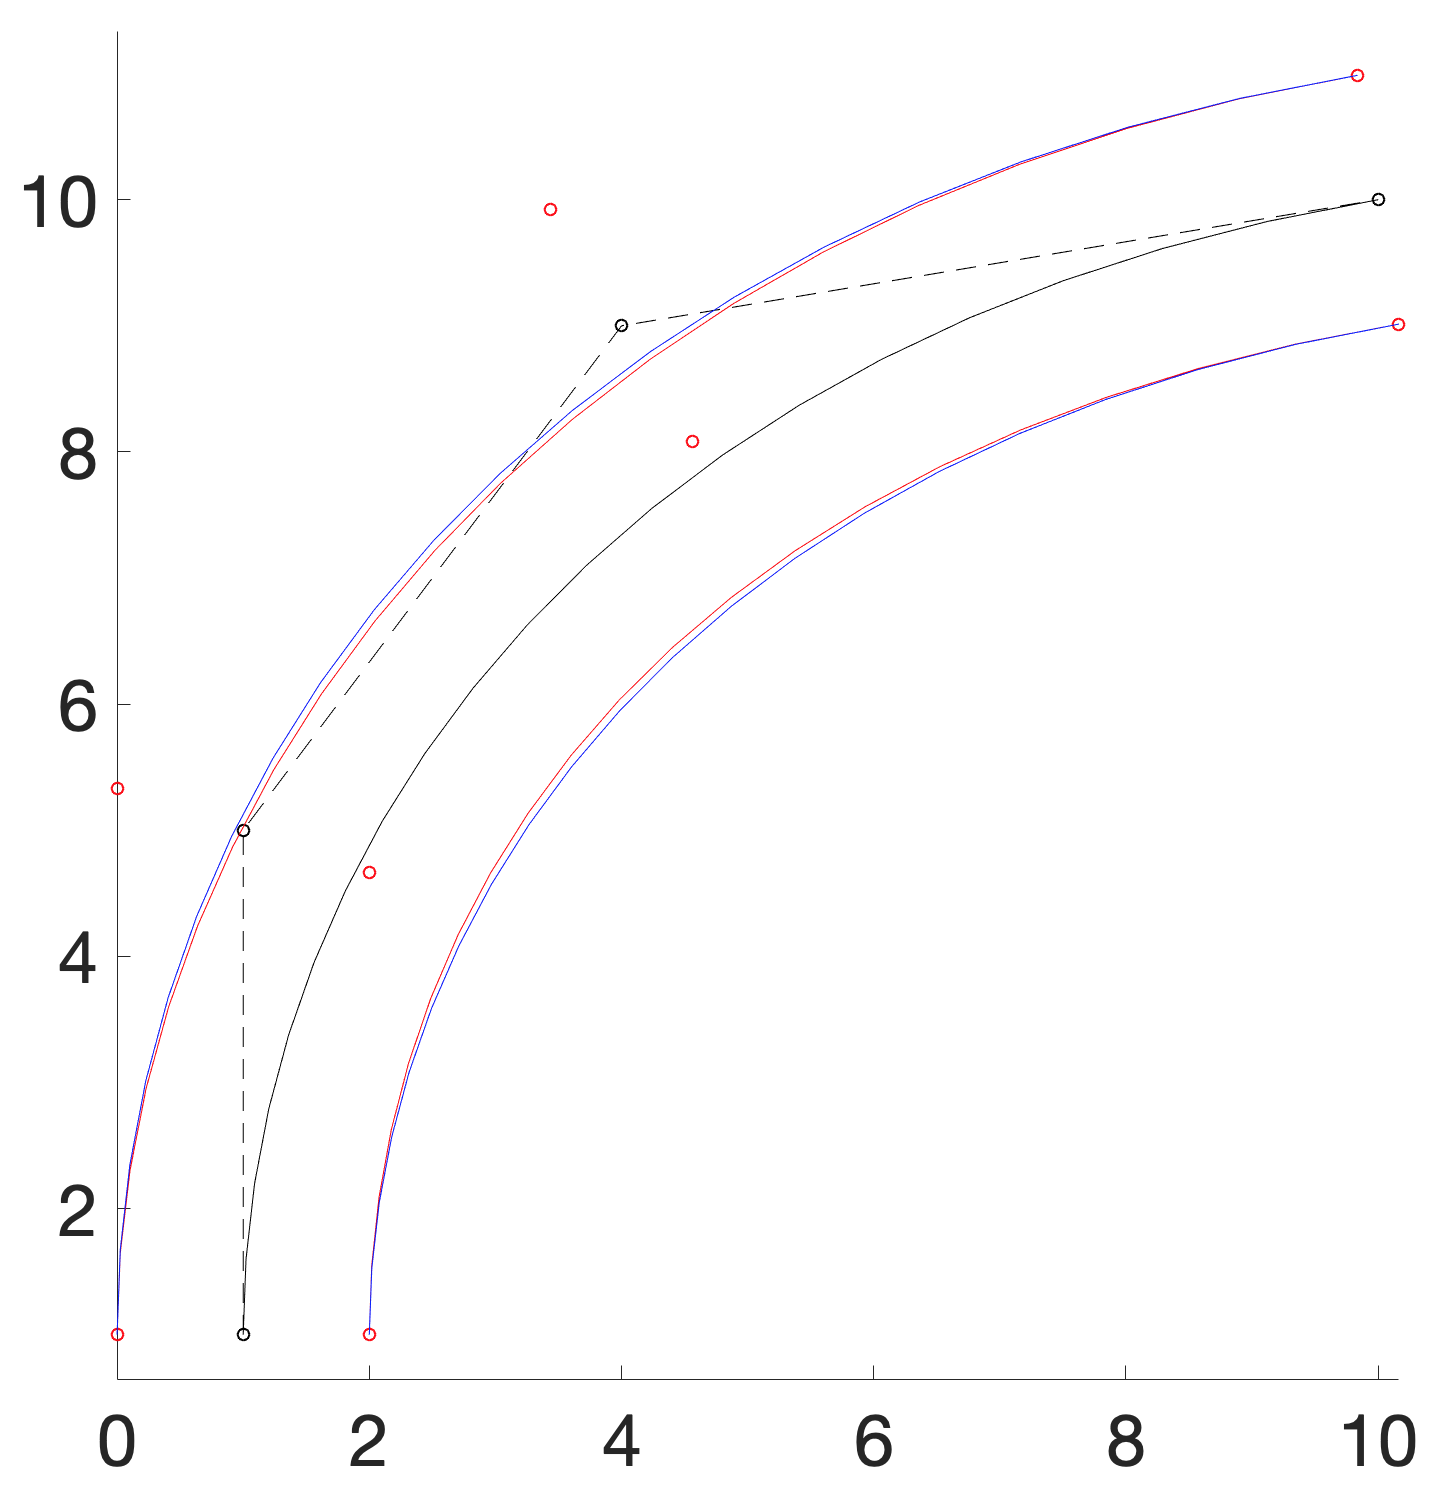
\includegraphics[width=60mm]{b1.png} &   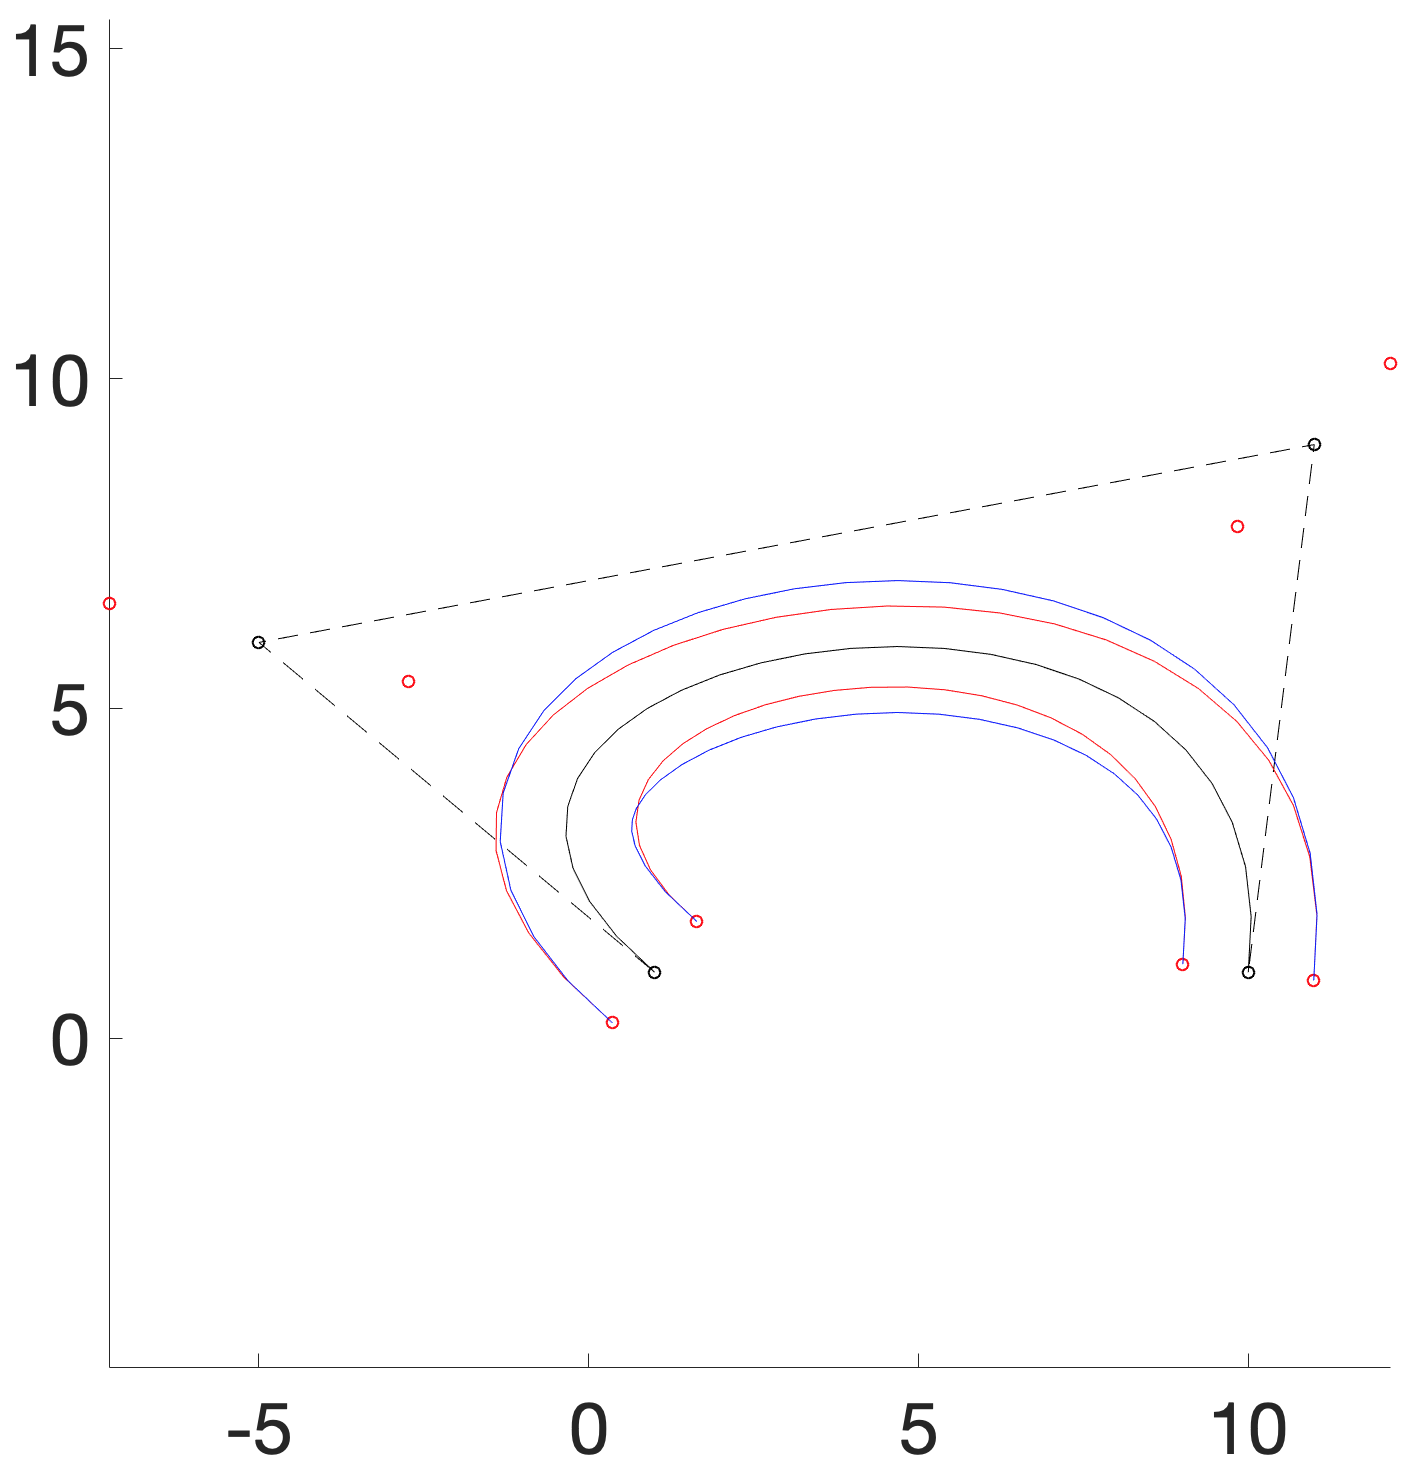
\includegraphics[width=60mm]{b2.png} \\
 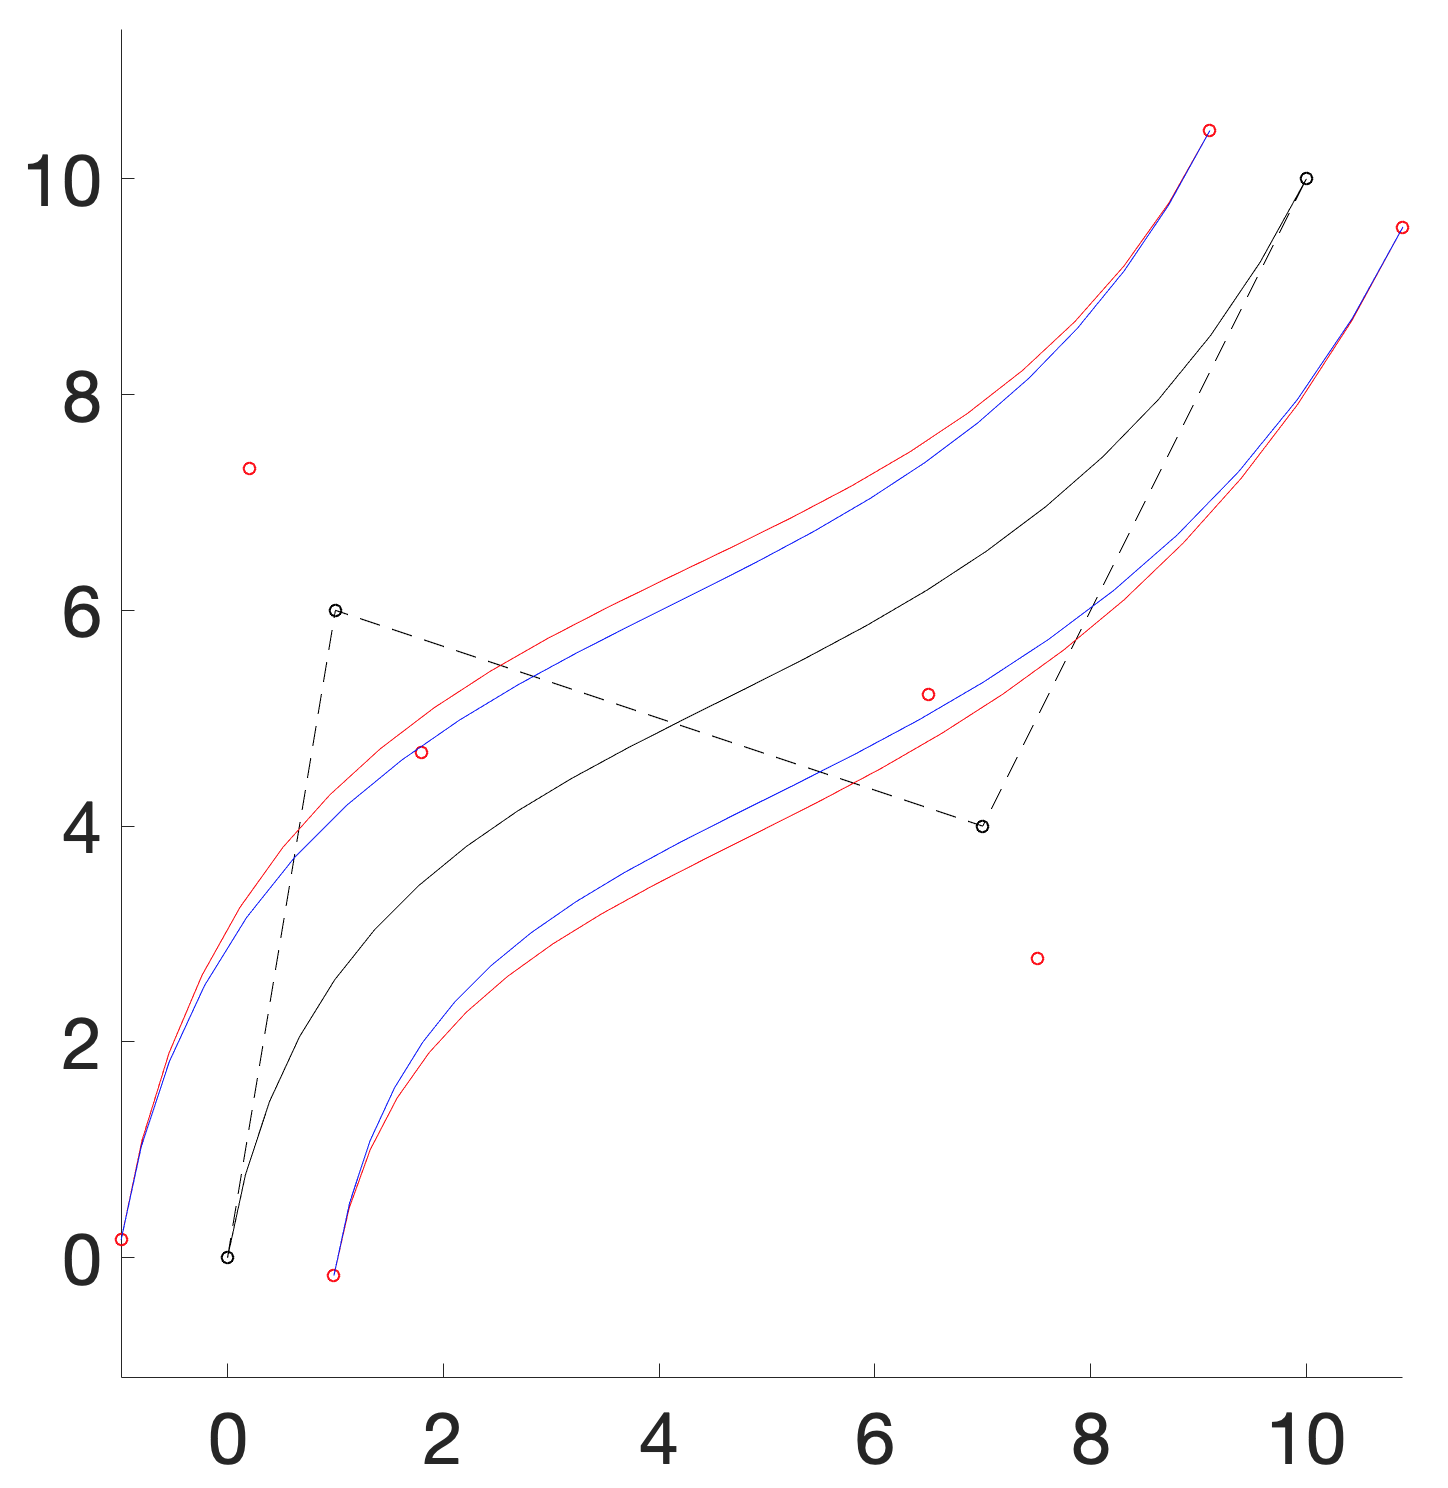
\includegraphics[width=60mm]{b3.png} &   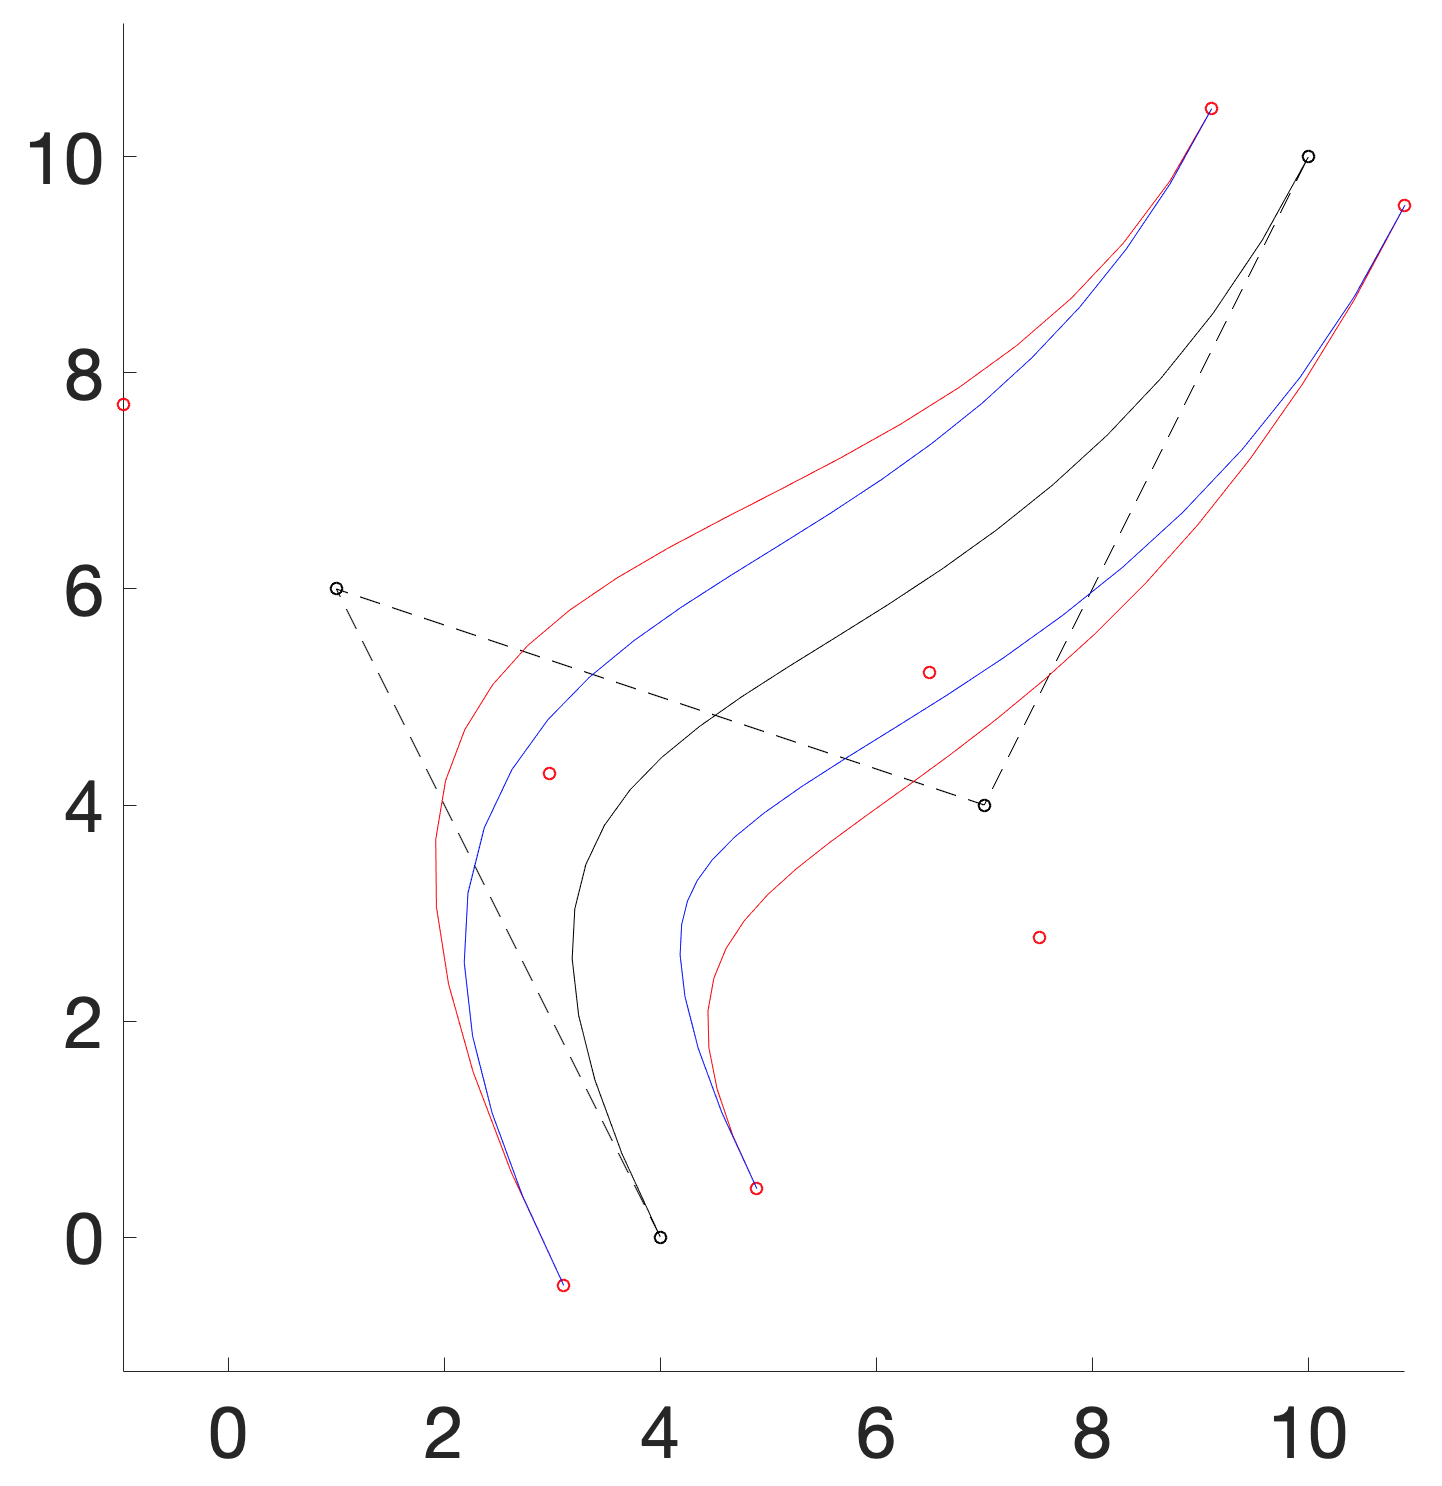
\includegraphics[width=60mm]{b4.png}
\end{tabular}
\caption{Comparison of two methods for approximating parallel Bezier curves. In black: the progenitor curve with its defining control points shown as circles connected by dashed lines. In red: approximation using the Tiller-Hanson method, with the associated control points shown as circles. In blue: approximation using a purely numerical method. This method was chosen for the vector map software.}
\label{fig:approx}
\end{figure}

Computing parallel linear and circular curves is trivial, because the resulting curves are also linear or circular. However, a curve parallel to a Bezier curve is not another Bezier curve. To the authors' knowledge, only approximation methods exist for solving this problem. Two approximation methods were compared, which is illustrated in Figure \ref{fig:approx}. The first attempt was an implementation of the Tiller-Hanson method, which involves shifting the control points defining the progenitor curve. The accuracy of the approximation is dependent on the original arrangement of control points. Errors using Tiller-Hanson method could easily be on the scale of meters, which is unacceptable for a driving simulation. Because the vector map requires discrete coordinate values, an equation for a parallel curve was only a convenience. Therefore, a numerical approach was proposed which would guarantee accuracy (see Algorithm \ref{alg:bezier}).

\begin{algorithm}
\caption{Compute the nearest point \textbf{Q} on the curve parallel to the Bezier curve defined by the control points $\textbf{P}_0, \textbf{P}_1, \textbf{P}_2, \textbf{P}_3$, evaluated at $t$, at a distance $d$ from the progenitor curve.}
\begin{algorithmic}
\REQUIRE $0 \leq t \leq 1$ and $\textbf{P}_n = (P_{xn}, P_{yn})$ and $d \geq 0$
\STATE $\textbf{B} \leftarrow (1-t)^3\textbf{P}_0+3(1-t)^2t\textbf{P}_1+3(1-t)t^2\textbf{P}_2+t^3\textbf{P}_3$
\STATE $d\textbf{B} \leftarrow 3(1-t)^2(\textbf{P}_1-\textbf{P}_0)+6(1-t)t(\textbf{P}_2-\textbf{P}_1)+3t^2(\textbf{P}_3-\textbf{P}_2)$
\STATE $\theta \leftarrow \arctan(dB_x, ~ dB_y)$
\STATE $\textbf{Q} \leftarrow (B_x + d \times \sin\theta, ~ B_y - d \times \cos\theta)$
\end{algorithmic}
\label{alg:bezier}
\end{algorithm}

\subsubsection{Software Design Patterns}

\section{Verification and Validation}
\label{section:VerificationAndValidation}
% Explain how you verified and validated your requirements. This can include such methods as unit tests, integration tests and system tests. Again, this chapter is as long as it needs to be.
% Remember, in regard to the learning goals this course is not about theory. We know that you know how to properly engineer an embedded system. Here you should offer evidence that you can also apply that knowledge. Of the learning goals in the course these are the ones that we believe will definitely be covered by this chapter:
% Goal 6. Working through all aspects of an engineering development process: You can for instance motivate the use of different test processes for different parts of your design; justify and prove the use of different levels of attention to ensuring the completeness, correctness and consistency of different types of requirements (for instance those that are mission-critical or related to safety and security); etc.
% Goal 9. Apply a fundamental test process: You can for instance provide evidence on the different types of errors, faults and failures logged throughout the project; motivate why the used verification and validation methods are appropriate for the problem at hand; discuss what verification and validation would have been appropriate but were not possible to apply (for instance destructive testing); etc.

\subsection{Vector Maps}

\section{Results}
\label{section:Results}
% Test results.  Factual findings. Does the final product fulfill the requirements? Relate / refer back to your requirements section.
% Remember, in regard to the learning goals this course is not about theory. We know that you know how to properly engineer an embedded system. Here you should offer evidence that you can also apply that knowledge. Of the learning goals in the course these are the ones that we believe will definitely be covered by this chapter:
% Goal 7. Designing and implementing prototypes: You can for instance show how your effort was able to address the most important goals of your project sponsor; justify the effort of creating the prototype in regard to its cost and time to finish; etc.



\section{Discussions and Conclusion}
\label{section:DiscussionAndConclusion}
%Reflect upon your results, highlighting what you have achieved.
%Then review your results a little more critically:
%Were they reasonable / good / poor / ultimately unrelated to solving the
%problem you started with?
%What could have been done differently to improve the outcome?
%How does your results relate to similar works?

\section{Future Work}
\label{section:FutureWork}
%Suggest potential leads and/or needs to solve / better solve the problem. Identify
%areas that can be developed. Highlight any areas of potential growth, or aspects
%that can be built on.





\bibliography{mybib}
%%\bibliographystyle{IEEEtran}
\bibliographystyle{myIEEEtran}



\end{document}
